\documentclass[letterpaper,onecolumn,titlepage]{Ythesis}
\usepackage[utf8]{inputenc}
\usepackage{tikz}
\usetikzlibrary{cd}
\usepackage{array,multirow}
\usepackage{subcaption}
\usepackage{subfiles}
\usepackage{url}
\usepackage{amsmath}
\usepackage{amssymb}
\usepackage{float}
\usepackage{diagbox}
\usepackage{graphicx}
\usepackage[backend=bibtex, style=numeric-comp]{biblatex}
\bibliography{glasslab_viz}
\title{Make any stupid plot you want}
\author{Hannah Aizenman}
\committee{Dr. Michael Grossberg (Advisor), Dr. Robert Haralick, Dr. Lev Manovich, Dr. Huy Vo}
\submitted{}
\abstract{}

\begin{document}
\makefrontmatter

\section{Introduction}
\label{sec:introduction}
\begin{figure}
    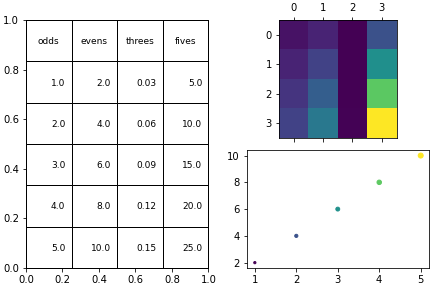
\includegraphics[width=.5\textwidth]{figures/intro/viz_same.png}
    \caption[]{Implicit in visualization is the assumption that these three representations of data are equivalent, specifically that the measurements within a variable and relations of the measurements of each variable are preserved. }
    \label{fig:viz_same}
\end{figure}

\subsection{Thesis statement}
We define a visualization as a transform from data to graphic that preserves the topology of the data and the properties of the measurement type. In fig~\ref{fig:viz_same}, we implicitly assume that the translation from table to heatmap has preserved the order of observations (the rows) and that the perceptually uniform sequential colormap has been applied such that the ordering relation on floats matches the ordering on the colormap (darker colors map to larger numbers). We also make this assumption about color in the scatter map, and that the translation to size and position on screen also respect the ordering on floats. In this work, we propose to mathematically describe the transform of data to visual space such that we can make explicit the implicit topology and types visualizations preserve. We then propose a new architecture for the Python visualization library Matplotlib \cite{hunterMatplotlib2DGraphics2007} based on these descriptions because the Matplolib artist layer is analogous to the transforms. 

\subfile{sections/math}
\printbibliography
\end{document}